\documentclass[a4paper]{report}

\usepackage[utf8]{inputenc}
\usepackage[english]{babel}
\usepackage[T1]{fontenc}
\usepackage{textcomp}
\usepackage[]{amsthm} 
\usepackage[]{amssymb}
\usepackage{amsmath}
\usepackage{graphicx}
\usepackage{float}
\usepackage{soul}
\usepackage{color}
\usepackage{bm}
\usepackage{listings}
\usepackage{xcolor}
\usepackage{enumitem}
%\usepackage{xfrac}
\usepackage[normalem]{ulem}
\usepackage{mathtools}


% ~~~~ no indent per paragraph ~~~~ 
\usepackage[parfill]{parskip}


\usepackage[colorlinks=true, linkcolor=blue]{hyperref}

\usepackage{tikz}
\usetikzlibrary{trees}
\usetikzlibrary {fit,shapes.geometric} % W: Command terminated with space. (1)
\usetikzlibrary {automata} % W: Command terminated with space. (1)
\usetikzlibrary{arrows.meta}
\usepackage{multicol}

\usepackage{algorithm}
\usepackage[noend]{algpseudocode}
\usepackage{caption}

% ~~~~ for subfigs ~~~~
\usepackage{subcaption}

\usepackage{pgfplots}
\pgfplotsset{compat = newest}

\usepackage{geometry}
\geometry{legalpaper, margin=1in}

\renewcommand{\labelitemii}{$\circ$}
\renewcommand{\labelitemiii}{$\star$}
\renewcommand{\labelitemiv}{$>$}

% figure support
\usepackage{import}
\usepackage{xifthen}
\pdfminorversion=7
\usepackage{pdfpages}
\usepackage{transparent}
\newcommand{\incfig}[1]{%
    \def\svgwidth{\columnwidth}
    \import{./figures/}{#1.pdf_tex}}

% Newline for algorithm psuedo
\newcommand{\algrule}[1][.2pt]{\par\vskip.5\baselineskip\hrule height #1\par\vskip.5\baselineskip}

% -------- Listings/XColor Settings --------
\definecolor{codegreen}{rgb}{0,0.6,0}
\definecolor{codegray}{rgb}{0.5,0.5,0.5}
\definecolor{codepurple}{rgb}{0.58,0,0.82}
\definecolor{backcolour}{rgb}{0.95,0.95,0.92}

\lstdefinestyle{mystyle}{
	backgroundcolor=\color{backcolour},
	commentstyle=\color{codegreen},
	keywordstyle=\color{magenta},
	numberstyle=\tiny\color{codegray},
	stringstyle=\color{codepurple},
	basicstyle=\ttfamily\scriptsize,
	breakatwhitespace=false,
	breaklines=true,
	captionpos=b,
	keepspaces=false,
	numbers=left,
	numbersep=5pt,
	showspaces=false,
	showstringspaces=false,
	showtabs=false,
	tabsize=4
}

\lstset{style=mystyle}

% -------------- Doc Start -------------------



\pdfsuppresswarningpagegroup=1

\title{\Huge{Sobel Filter on FPGA}}
\author{\textbf{Authors:} \\WhisperingRock \\ \\ \textbf{Professor:} \\}
\date{Class:\\ \small{Quarter}: \\ \today}

\begin{document}
    \maketitle
	\phantomsection
	\addcontentsline{toc}{section}{\contentsname}
	\tableofcontents

	\chapter{Theory of the Sobel Operator}

		\section{Grayscale Operator}
		This implementation requires that the RBG image (\hl{TODO} img type) 
				be flattened into a single intensity value (a grayscale value). 
				This can be done with a few methods.

			\begin{itemize}
				\item Average : $$p = \frac{R + G + B}{3}$$
				\item \href{https://en.wikipedia.org/wiki/Rec._709}{ITU-R B.709 Luminance}
					\[p = 0.2126 R + 0.7152 G + 0.0722 B\]
			\end{itemize}
 
			I opt'd to use Luminance for its accepted standard.

		\section{Sobel Operator}	

			Uses two 3x3 kernels which are convolved with the original 
			(grayscale) image to calculate approximations of the derivatives. 
			Each kernel, one for horizontal change and one for vertical change, 
			performs a low pass Gaussian filtering [1 2 1] as well a discrete
			differentiation [+1 0 -1] on each pixel of the image.

			 \[
			 	\bf{G_x} =
			 	\begin{bmatrix}
			 		+1 & 0 & -1 \\
			 		+2 & 0 & -2 \\
			 		+1 & 0 & -1
			 	\end{bmatrix}
				=
			 	\begin{bmatrix} 1 \\ 2 \\ 1 \end{bmatrix}
			 	\begin{bmatrix} +1 & 0 & -1 \end{bmatrix}
			\]

			\[ 
				\bf{G_y} =
				\begin{bmatrix}
					+1 & +2 & +1 \\
					0 & 0 & 0 \\
					-1 & -2 & -1
				\end{bmatrix}
				= 
				\begin{bmatrix} +1 \\ 0 \\ -1 \end{bmatrix}
				\begin{bmatrix} 1 & 2 & 1 \end{bmatrix}
			\]
 
			Consider the resulting components : 
			\begin{itemize}
				\item Magnitude : $$\bf{G} = \sqrt{\bf{G_x}^2 + \bf{G_y} ^ 2}$$
				\item Direction of gradient : $$\bf{\Theta} = \arctan{\left(\frac{G_y}{G_x}\right)}$$
			\end{itemize}

			The results of the operator produce a cheap edge detector that 
			performs some smoothing while retaining a DC gain of 1.
			For the scope of this project, I'm only using the magnitude.

	\chapter{System Architecture}

	\chapter{FPGA IP}
	
		\section{Line Buffer}

			The LineBuffer is designed to \ldots
			\begin{itemize}
				\item incrementally collect individual input pixel values 
						into the internal storage, using \textit{DIN\_AVAIL} 
						and \textit{DIN}, on each clock cycle. \textit{DIN\_AVAIL}
						enables writes while also moving the write pointer to the 
						next position.
				\item always output a 3 pack of neighbor pixels to \textit{DOUT},
						only updating and shifting on a clock'd \textit{DOUT\_AVAIL}.

				\item naturally rollover internal readPtr and writePtr to
						512 count (pixels) or reset to zero using \textit{RST}.
						One might consider the buffer circular using the rollover.
			\end{itemize}


			Notes:
			\begin{itemize}
				\item Need at least three writes at or ahead of readPtr before 
					using output data to avoid reading junk.
			\end{itemize}
			
			\begin{figure}[H]
				\centering
				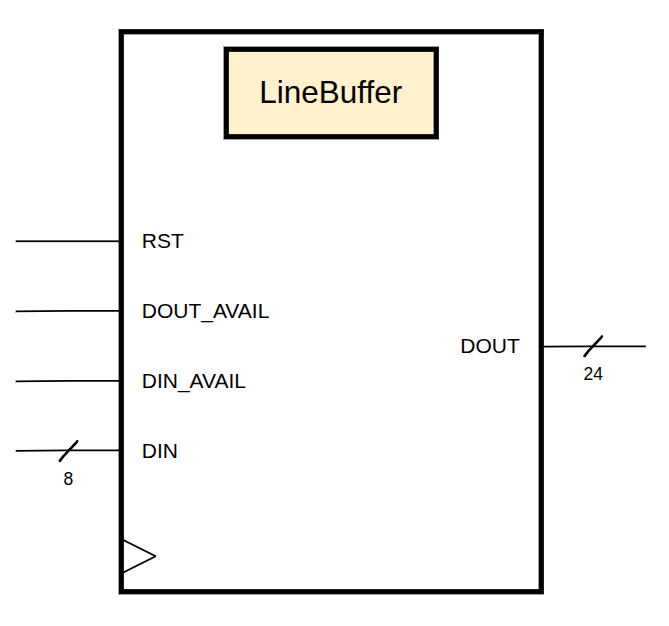
\includegraphics[width=0.3\textwidth]{../01_supporting/linebuffer/block.png}
				\caption{LineBuffer Block}
				\label{fig:lb_block}
			\end{figure}

			\begin{figure}[H]
				\centering
				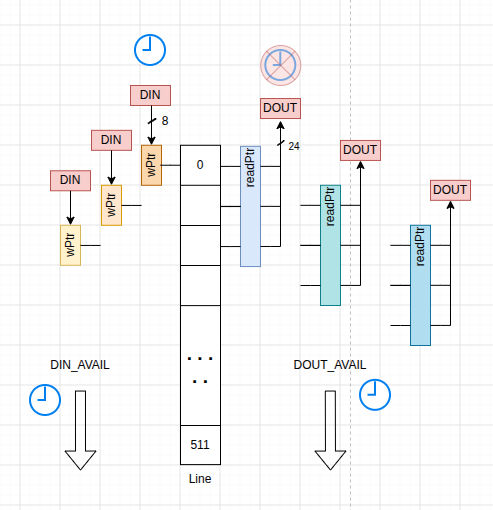
\includegraphics[width=0.5\textwidth]{../01_supporting/linebuffer/visual.png}
				\caption{LineBuffer Visualized}
				\label{fig:lb_visual}
			\end{figure}

			\begin{figure}[H]
				\centering
				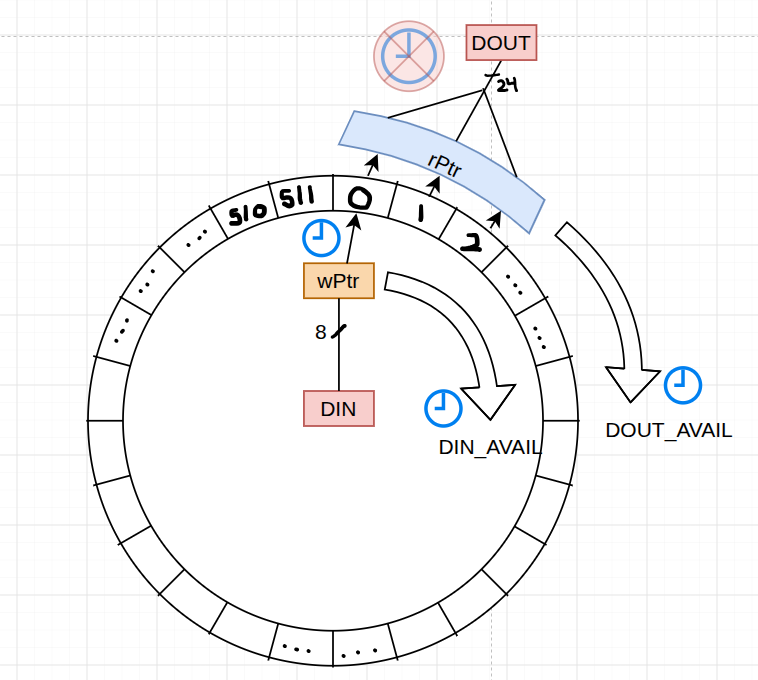
\includegraphics[width=0.5\textwidth]{../01_supporting/linebuffer/visual1.png}
				\caption{LineBuffer Visualized as Circular}
				\label{fig:lb_visual_circ}
			\end{figure}

			\begin{figure}[H]
				\centering
				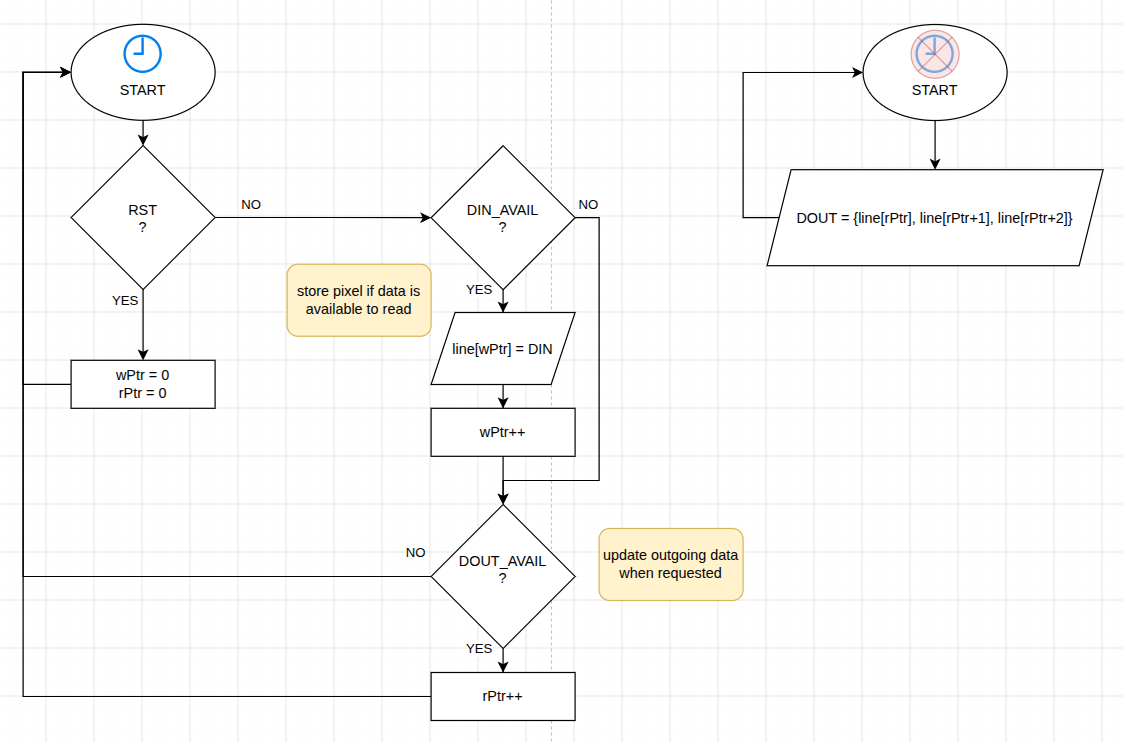
\includegraphics[width=0.7\textwidth]{../01_supporting/linebuffer/flow.png}
				\caption{LineBuffer Flowchart}
				\label{fig:lb_flow}
			\end{figure}

			\begin{figure}[H]
				\centering
				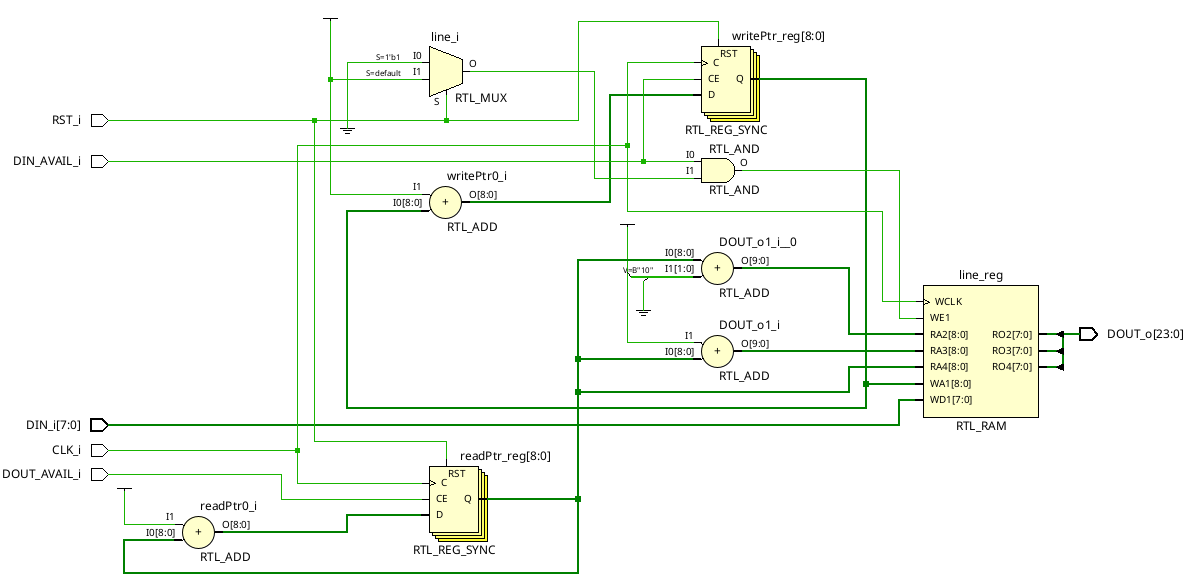
\includegraphics[width=0.8\textwidth]{../01_supporting/linebuffer/rtl.png}
				\caption{LineBuffer RTL}
				\label{fig:lb_rtl}
			\end{figure}	

			Code : 
			\begin{itemize}
				\item \texttt{LineBuffer.sv} \ref{code:linebuff}
				\item \texttt{LineBuffer\_tb.sv} \ref{testcode:linebuff}
			\end{itemize}

		\newpage
		\section{Convolution}

			The Convolution module is designed to \ldots
			\begin{itemize}
				\item Perform a single matrix multiplication as part of
						convolving the image with the kernel filter. 
			\end{itemize}

			The kernels used were :

			\textbf{Unity Gain Box Blurr}
			\[
				k = 
					\frac{1}{9}
					\begin{bmatrix}
						1 & 1 & 1 \\
						1 & 1 & 1 \\
						1 & 1 & 1 
					\end{bmatrix}
			\] 

			\textbf{Sobel X-axis}
			\[
				k = 
					\begin{bmatrix}
						1 & 0 & -1 \\
						2 & 0 & -2 \\
						1 & 0 & -1 
					\end{bmatrix}
			\] 

			\textbf{Sobel Y-axis}
			\[
				k = 
					\begin{bmatrix}
						 1  &  2  &  1 \\
					 	 0  &  0  &  0 \\
						-1  & -2  & -1 
					\end{bmatrix}
			\] 


			\subsection{Design}

				\textbf{Always}:
				\[
					sum = \sum_{i=0}^{8} m[i] * k[i]
				\] 

				\textbf{CLK}:
				\[
					\text{\texttt{Result}} = 
					\begin{cases*}
						\text{\texttt{Result}} & , if $ \overline{\text{\texttt{MATRIX\_VALID}}}$ \\\\
						\begin{cases*}
							0 	& , if	$sum < 0$ 	\\
							255	& , if	$sum > 255$	\\
							\frac{sum}{div} & , else
						\end{cases*} & , if $\text{\texttt{MATRIX\_VALID}}$
					\end{cases*}
				\]\\ 

				\[
					\text{\texttt{RESULT\_VALID}} =  \text{\texttt{MATRIX\_VALID}}
				\] 


			\begin{figure}[H]
				\centering
				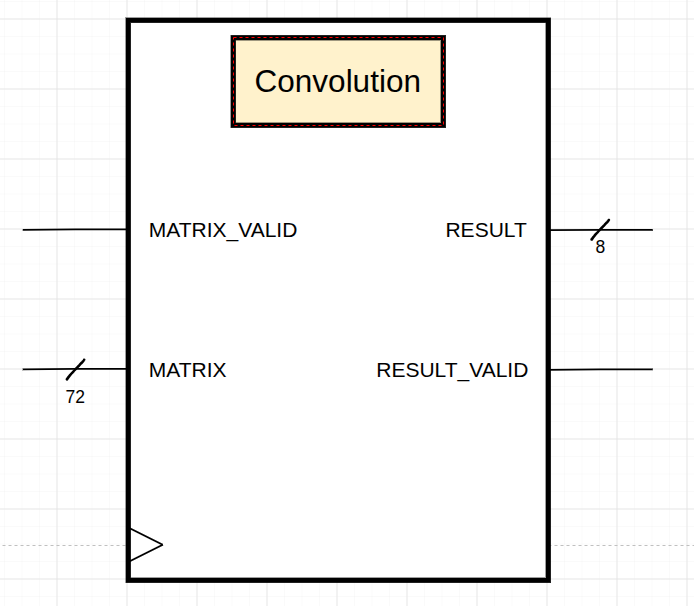
\includegraphics[width=0.3\textwidth]{../01_supporting/convolution/block.png}
				\caption{Convolution Block}
				\label{fig:conv_block}
			\end{figure}

			\begin{figure}[H]
				\centering
				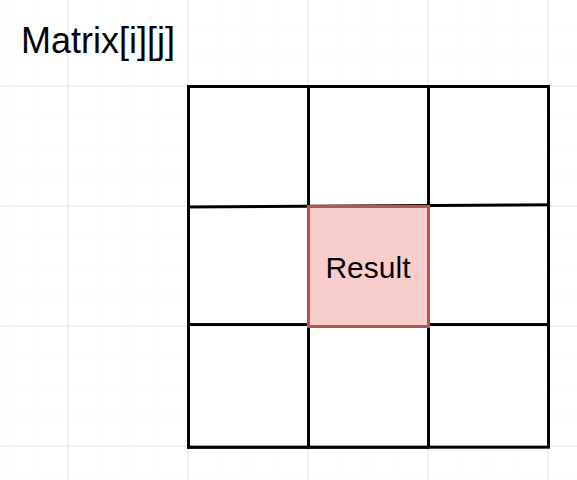
\includegraphics[width=0.3\textwidth]{../01_supporting/convolution/visual.png}
				\caption{Convolution Visualized}
				\label{fig:conv_visual}
			\end{figure}

			\begin{figure}[H]
				\centering
				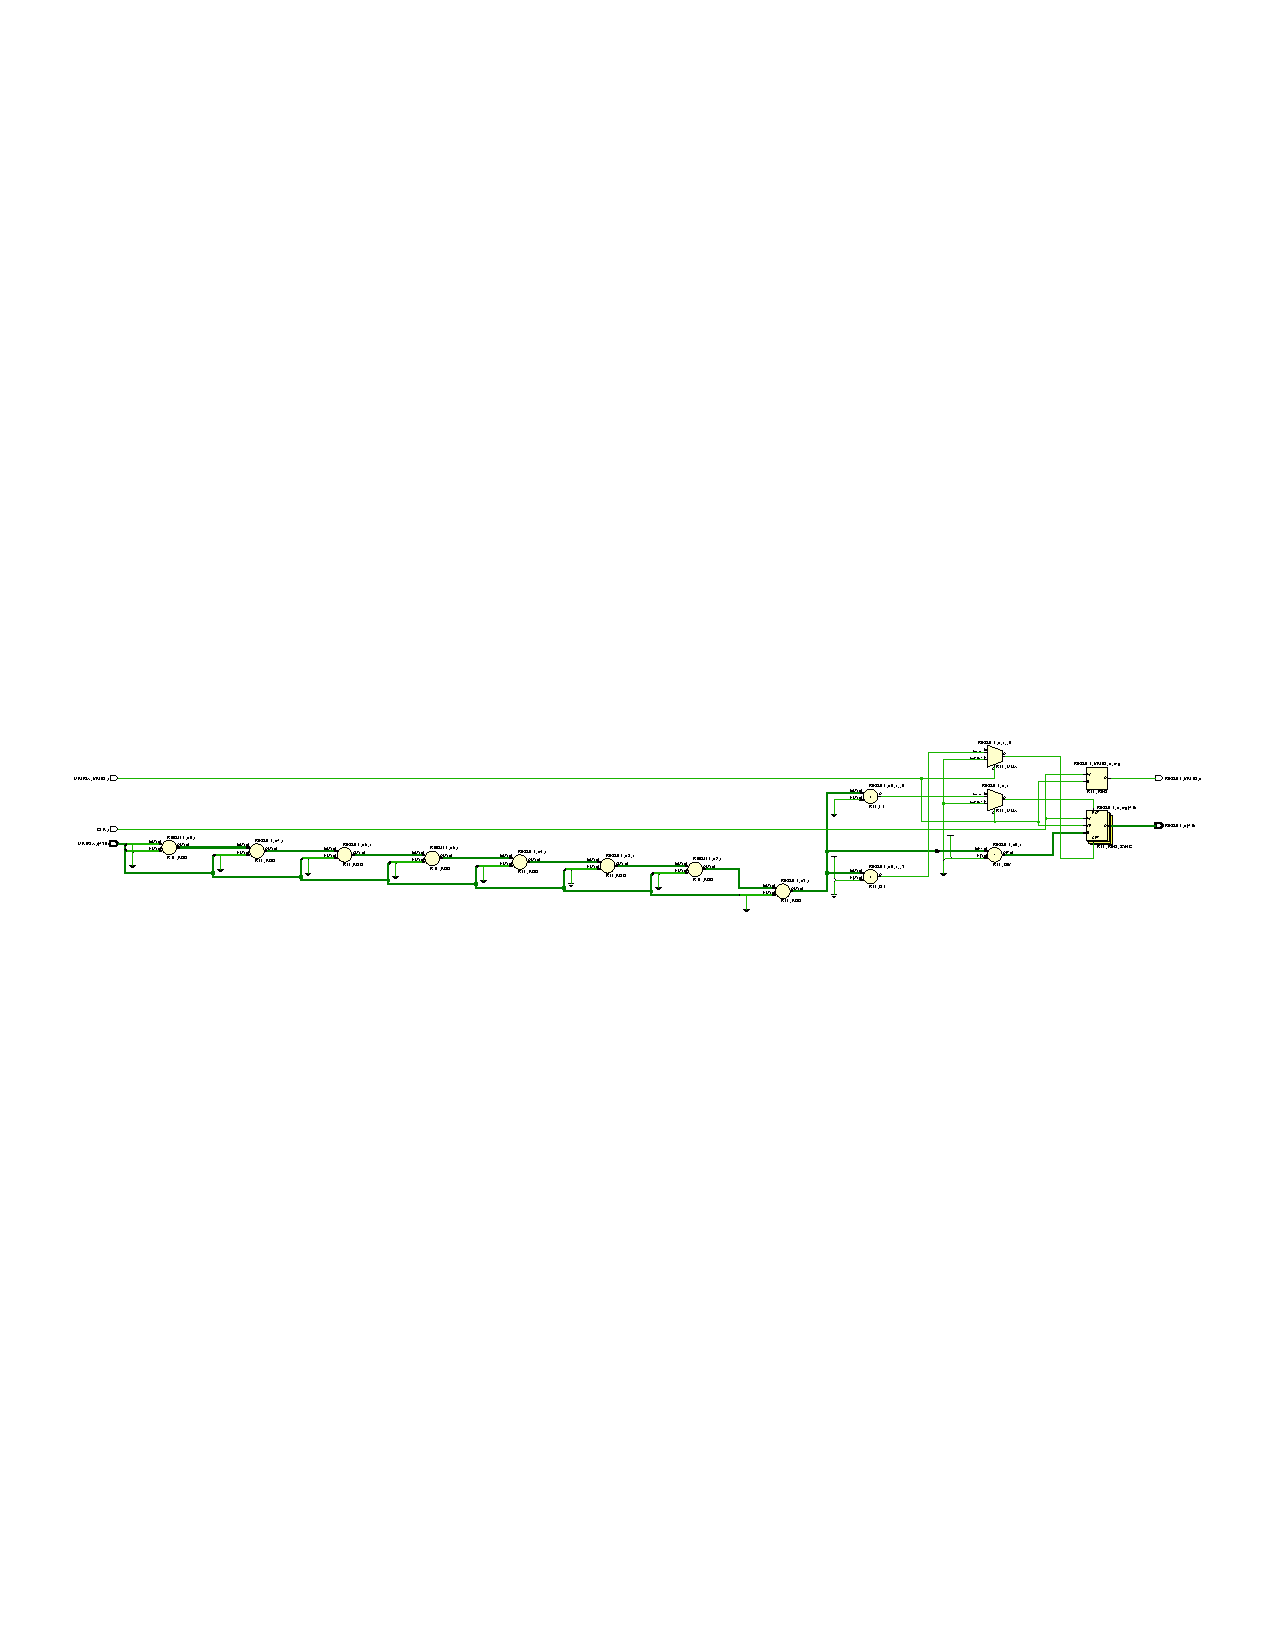
\includegraphics[
					angle			= 90,
					origin			= c,
					trim			= 5mm 90mm 5mm 90mm,
					clip,
					width			= 0.8\textwidth,
					keepaspectratio	= true
				]{../01_supporting/convolution/rtl.pdf}
				\caption{Convolution RTL}
				\label{fig:conv_rtl}
			\end{figure}

			Code : 
			\begin{itemize}
				\item \texttt{Convolution.sv} \ref{code:convolution}
				\item \texttt{Convolution\_tb.sv} \ref{testcode:convolution}
			\end{itemize}

		\newpage
		\section{Image Control Unit}

			The IMU is designed to :
			\begin{itemize}
				\item Orchestrate which LineBuffer is to receive incoming pixel data through the use of
						counters and indexers \texttt{pixelCounter} and \texttt{currWrLineBuff}. 
						\texttt{pixelCounter} is the current pixel for the row and \texttt{currWrLineBuff}
						indicates which LineBuffer is recieving the incoming data. 

				\item Orchestrate which LineBuffers are contributing to the exported 3x3 matrix window 
						through the use of counters and indexers \texttt{windowCounter} and \texttt{currRdLineBuff}. 
						\texttt{windowCounter} is the window's left-most pixel in reference to a row of pixels. Said 
						another way, incrementing this variable slides the 3x3 window right by one pixel and
						resets after reaching 511 pixels. \texttt{currRdLineBuff} controls which combination of 
						LineBuffer outputs are used to create the window s.t. incrementing this variable 
						shifts the 3x3 window down by one pixel. 

				\item Ensure there are at least three rows of pixel data in the buffer before sliding
						the output window. This is tracked using \texttt{currBufferedPixels} and the FSM
						logic.
			\end{itemize}

			\hl{NOTE} : I really need to use UVM encapsulation/sanitization for testing this module. 
						The read and write pointers do not line up and there is no way to erase
						the memory contents of the line buffers with reset. That would probably take
						a considerable effort to do such a thing\ldots

			\begin{figure}[H]
				\centering
				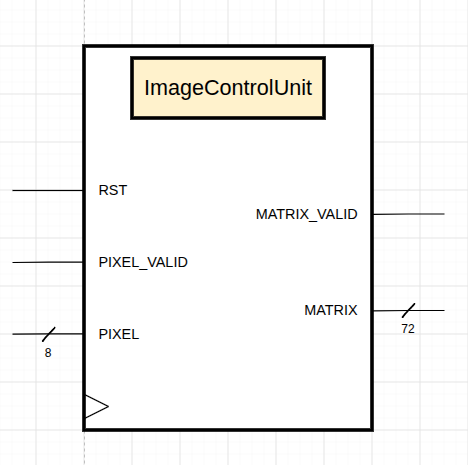
\includegraphics[width=0.3\textwidth]{../01_supporting/image_control_unit/block.png}
				\caption{IMU Block}
				\label{fig:imu_block}
			\end{figure}

			\begin{figure}[H]
				\centering
				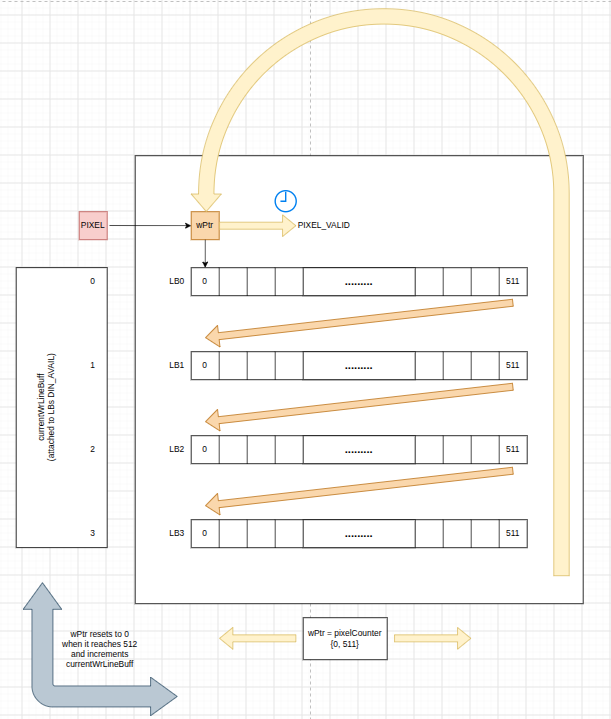
\includegraphics[width=0.6\textwidth]{../01_supporting/image_control_unit/visual_input.png}
				\caption{IMU Data Importing Visualized}
				\label{fig:imu_visual_import}
			\end{figure}

			\begin{figure}[H]
				\centering
				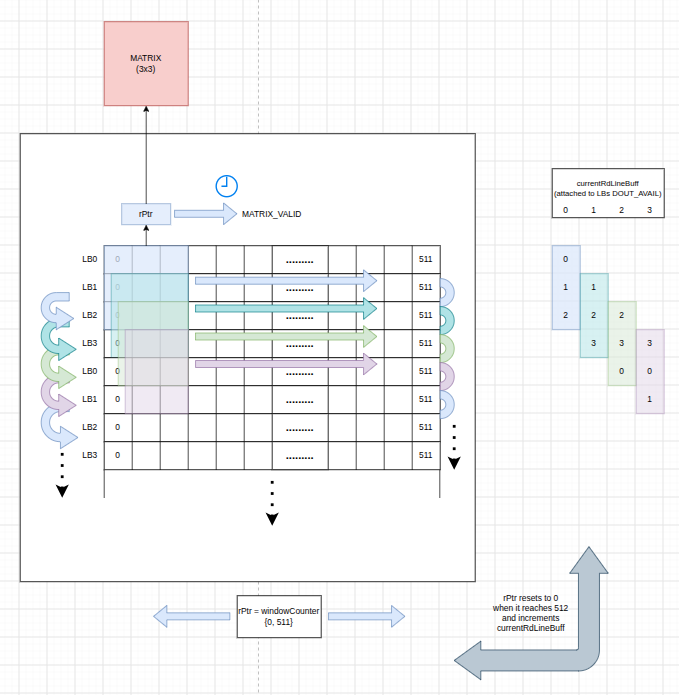
\includegraphics[width=0.6\textwidth]{../01_supporting/image_control_unit/visual_output.png}
				\caption{IMU Data Exporting Visualized}
				\label{fig:imu_visual_export}
			\end{figure}

			\begin{figure}[H]
				\centering
				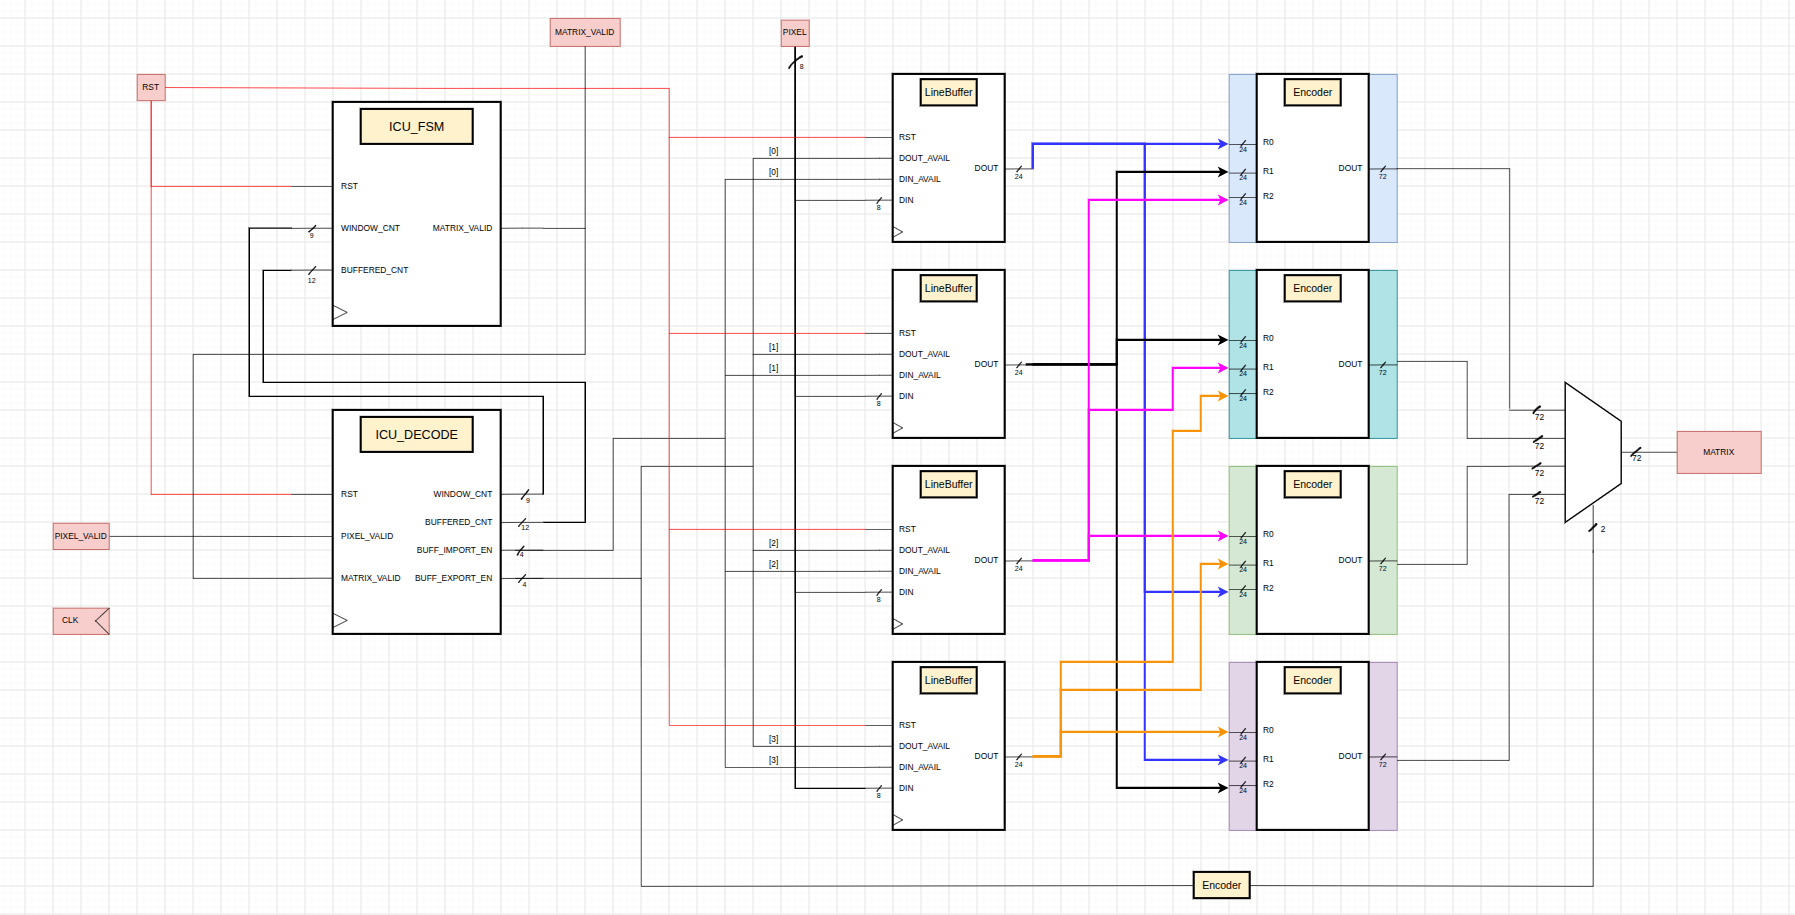
\includegraphics[width=1.0\textwidth]{../01_supporting/image_control_unit/visual_2.png}
				\caption{IMU Visualized in another way}
				\label{fig:imu_visual_2}
			\end{figure}

			\begin{figure}[H]
				\centering
				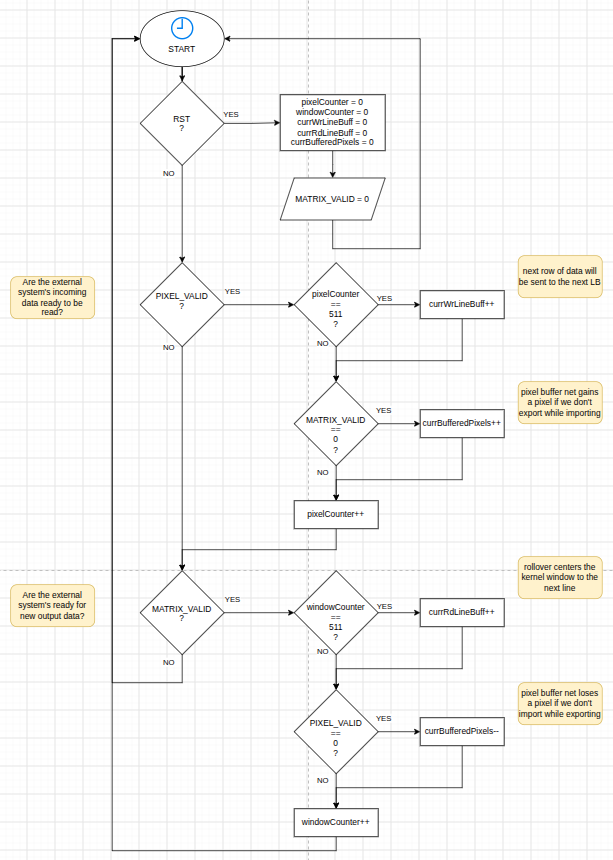
\includegraphics[width=0.8\textwidth]{../01_supporting/image_control_unit/flow_sync.png}
				\caption{IMU CLK Sync'd Flowchart}
				\label{fig:imu_flow}
			\end{figure}

			\begin{figure}[H]
				\centering
				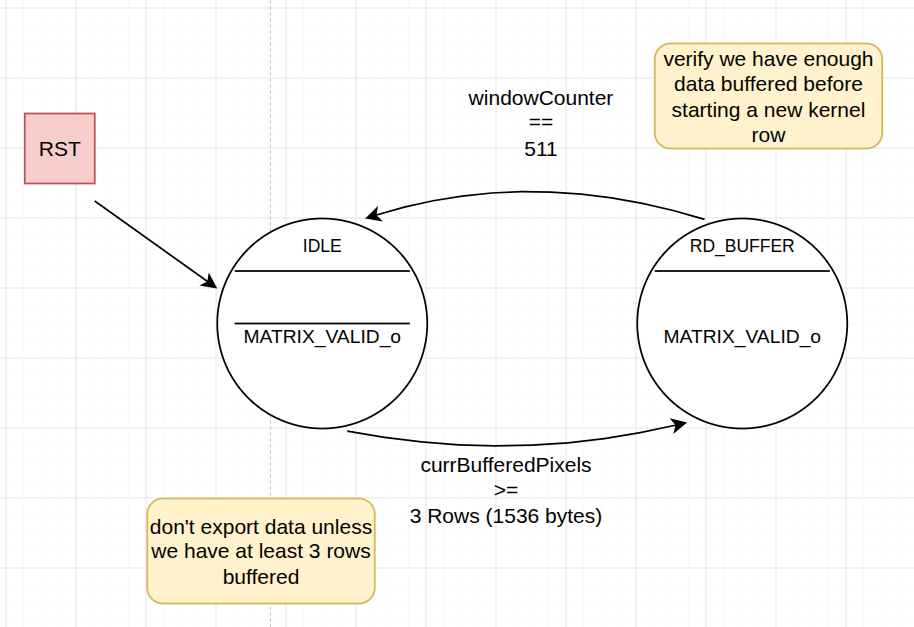
\includegraphics[width=0.6\textwidth]{../01_supporting/image_control_unit/fsm.png}
				\caption{IMU FSM}
				\label{fig:imu_fsm}
			\end{figure}

			\begin{figure}[H]
				\centering
				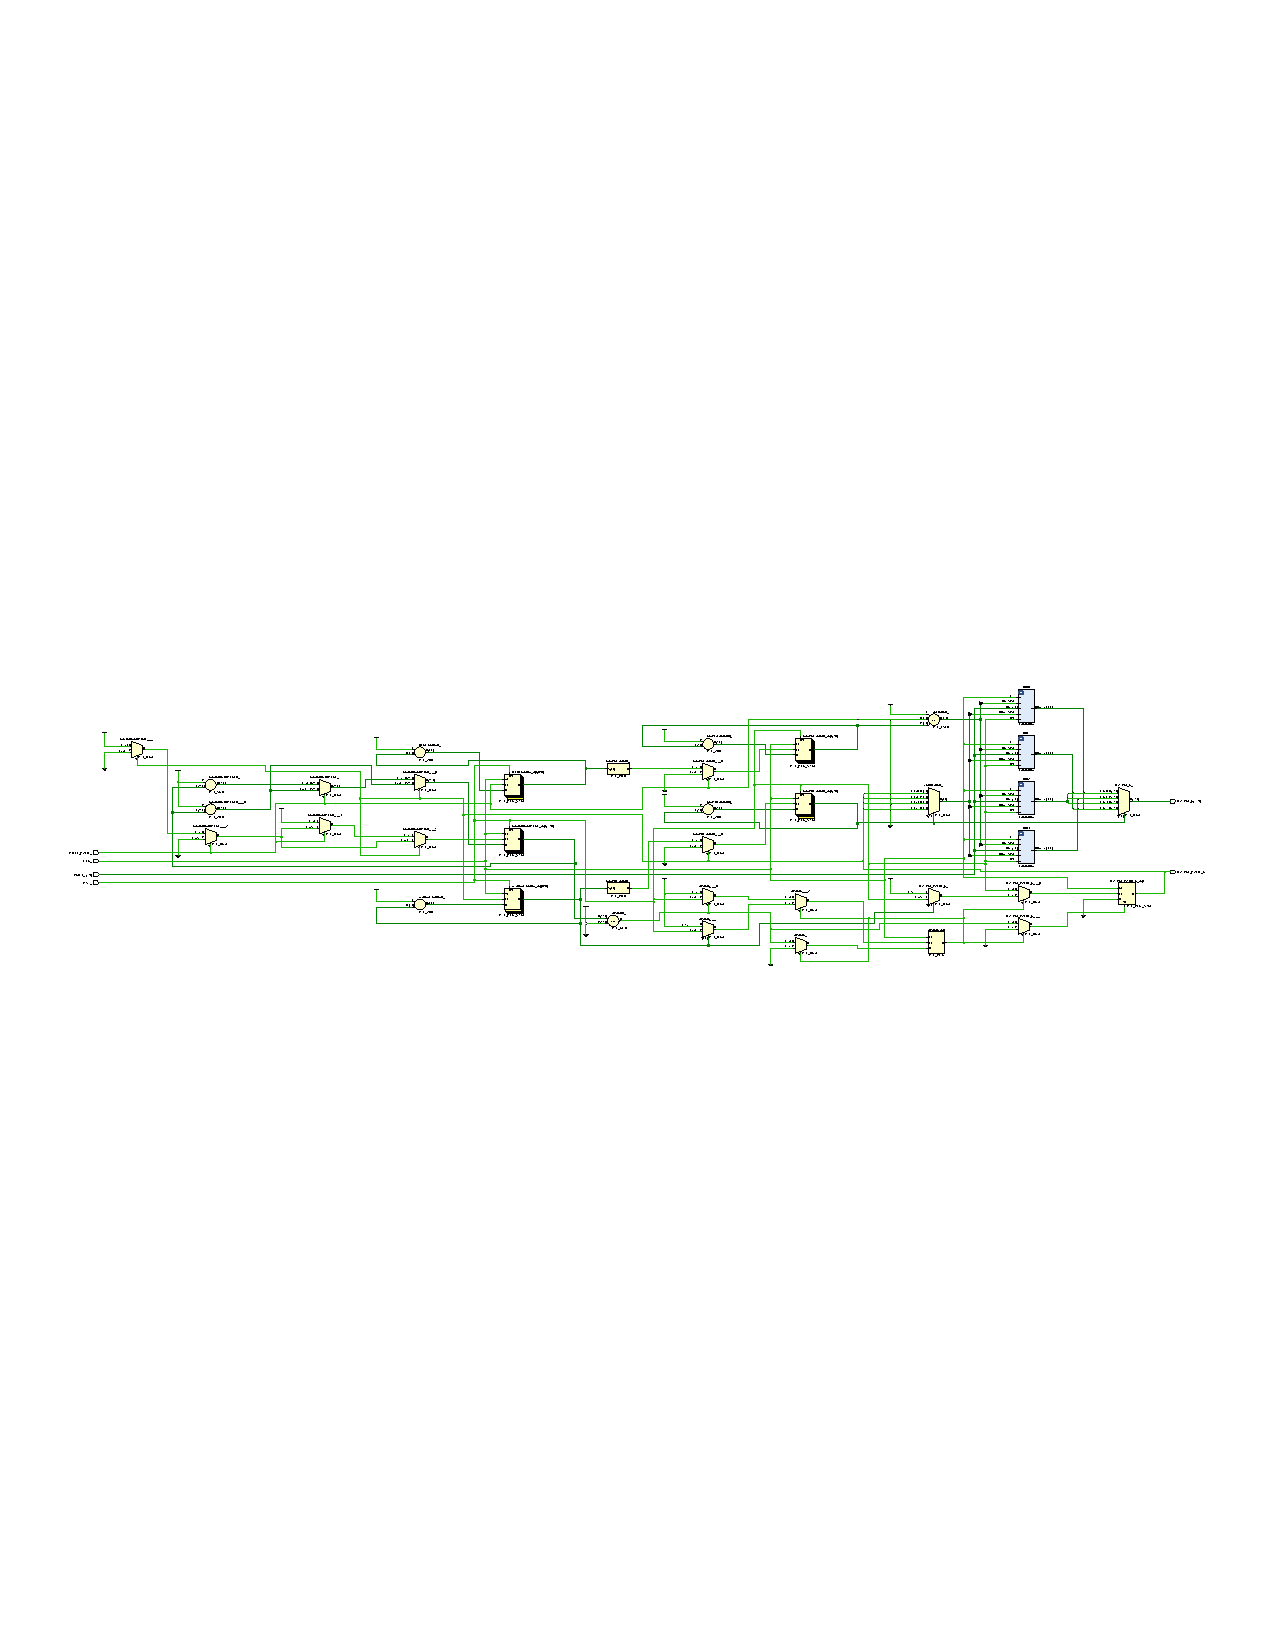
\includegraphics[
					angle			= 90,
					origin			= c,
					trim			= 5mm 90mm 5mm 90mm,
					clip,
					width			= 0.8\textwidth,
					keepaspectratio	= true
				]{../01_supporting/image_control_unit/rtl.pdf}
				\caption{IMU RTL}
				\label{fig:imu_rtl}
			\end{figure}
			
			Code : 
			\begin{itemize}
				\item \texttt{ImageControlUnit.sv} \ref{code:imu}
				\item \texttt{ImageControlUnit\_tb.sv} \ref{testcode:imu}
			\end{itemize}

		\newpage
		\section{Image Control Top}

			The Image Control Top module is designed to :
			\begin{itemize}
				\item \ldots
			\end{itemize}

			\begin{figure}[H]
				\centering
				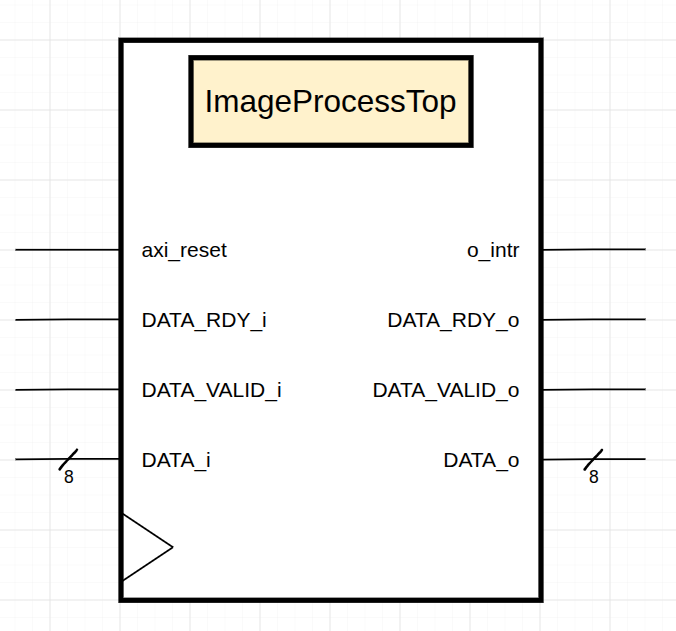
\includegraphics[width=0.3\textwidth]{../01_supporting/image_control_unit_top/block.png}
				\caption{IM Top Block}
				\label{fig:imu_top_block}
			\end{figure}

			\begin{figure}[H]
				\centering
				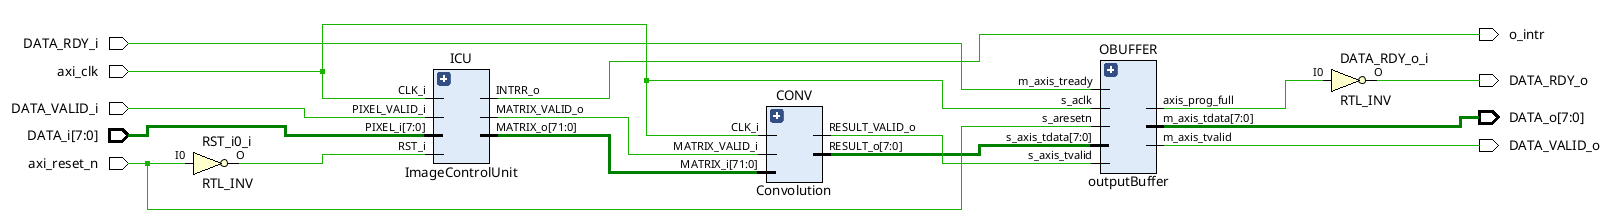
\includegraphics[width=0.9\textwidth]{../01_supporting/image_control_unit_top/rtl.png}
				\caption{IM Top Hardware}
				\label{fig:imu_top_rtl}
			\end{figure}

			\subsection{Output Buffer}

				The module now has a 2-depth FIFO output buffer, supplied by Vivado IP, but why?
				Well, the FIFO is useful because the filter pipeline could produce
				result pixels at a different rate than the downstream could
				accept them. Without the buffer, the convolution block could
				overwrite its previous result before it is read. Fortunately for us, 
				this scenario is more likely than the entire pipeline stalling out
				but that could still occur. 

				While the current simulation is not connecting the full indicator, 
				this will be useful for regulating the pipeline back pressure.

			\subsection{AXI Bus}

			\newpage
			\subsection{Design Questions}
				\subsubsection{Q: How many buffers should we initially fill?}

					The model needs at least three buffers filled to start the convolution
					and we only have four line buffers to fill so some potential 
					options are pre-filling three or all four line buffers. 
					Lets compare the sim results side by side :

					\begin{figure}[H]
						\centering
						\begin{subfigure}{1.0\textwidth}
							\centering
							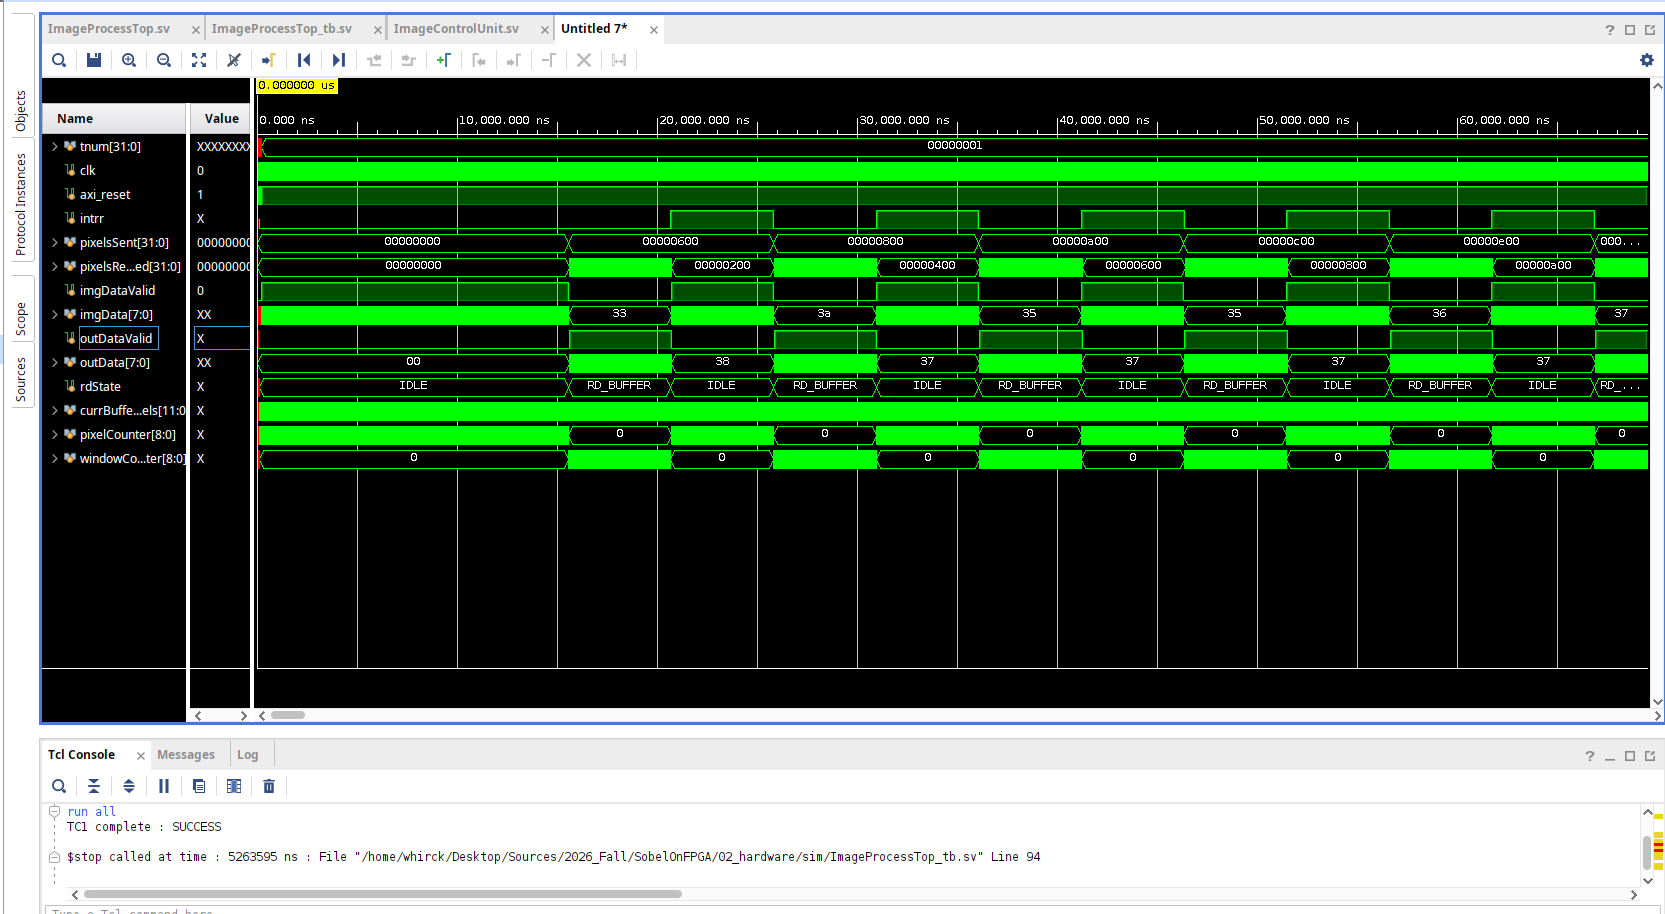
\includegraphics[
								width			= 0.8\textwidth,
								keepaspectratio	= true
							]{../01_supporting/image_control_unit_top/sim_3LB_wave.png}
							\caption{Macro waveform for 3 line buffers}
						\end{subfigure}
						\hfill
						\begin{subfigure}{1.0\textwidth}
							\centering
							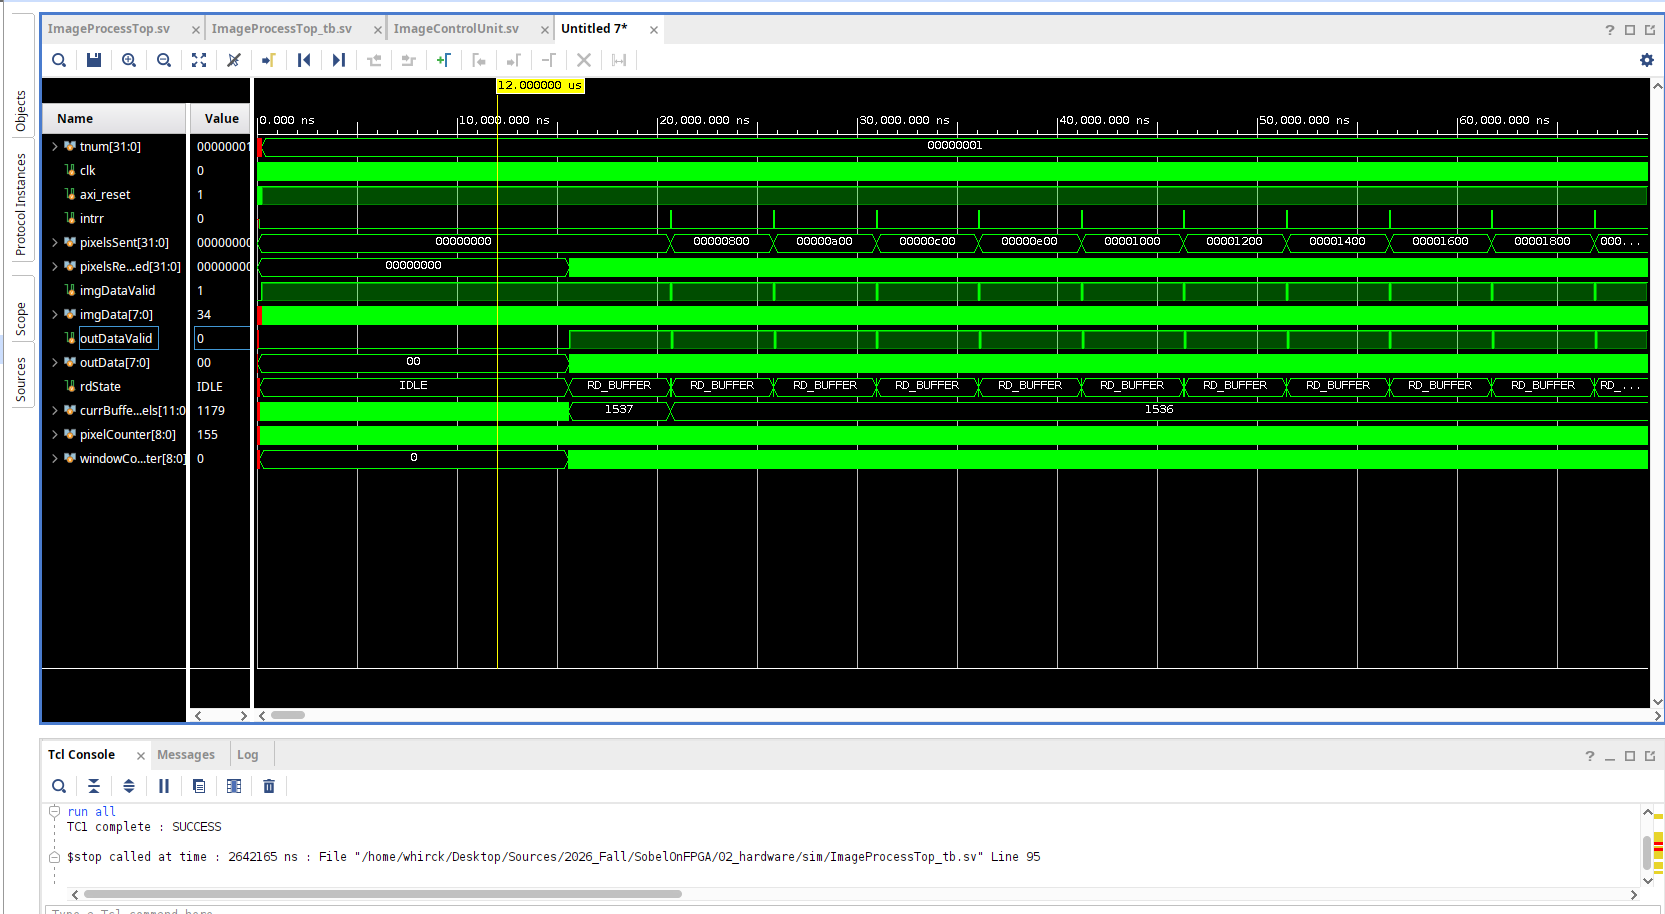
\includegraphics[
								width			= 0.8\textwidth,
								keepaspectratio	= true
							]{../01_supporting/image_control_unit_top/sim_4LB_wave.png}
							\caption{Macro waveform for 4 line buffers}
						\end{subfigure}
						\caption{Simulation between 3 and 4 prefilled LineBuffers}
						\label{fig:}
					\end{figure}	

					Observations between waveforms :
					\begin{itemize}
						\item \textbf{Timing} : It took the 3LBs 5.26 \texttt{ms} and 2.64 \texttt{ms} for 4LB 
							to complete the block blurr algorithm. It almost took twice as long 
							to do the entire process based off of a single 
							prefill. Thats big.

						\item \textbf{Read/Write} : 
							For 3LB, we are not importing
							in new values while writing nor are we exporting data
							while importing. This is also reflected in the states
							where we reside in one logic state for 512 reads or writes
							but not both. For 3LB, it seems we are always 
							waiting to read or write but never both. 

							For 4LB, it appears we briefly go into the \texttt{IDLE}
							state but largely remain in the \texttt{RD\_BUFFER} state.
							This somehow allows us to import AND export data at
							the same time, likely cutting down our compute time in
							the process. 
					\end{itemize}

					Given such large gap in performance between the two options, 
					lets take a closer look at what is going on here.

					\begin{figure}[H]
						\centering
						\begin{subfigure}{1.0\textwidth}
							\centering
							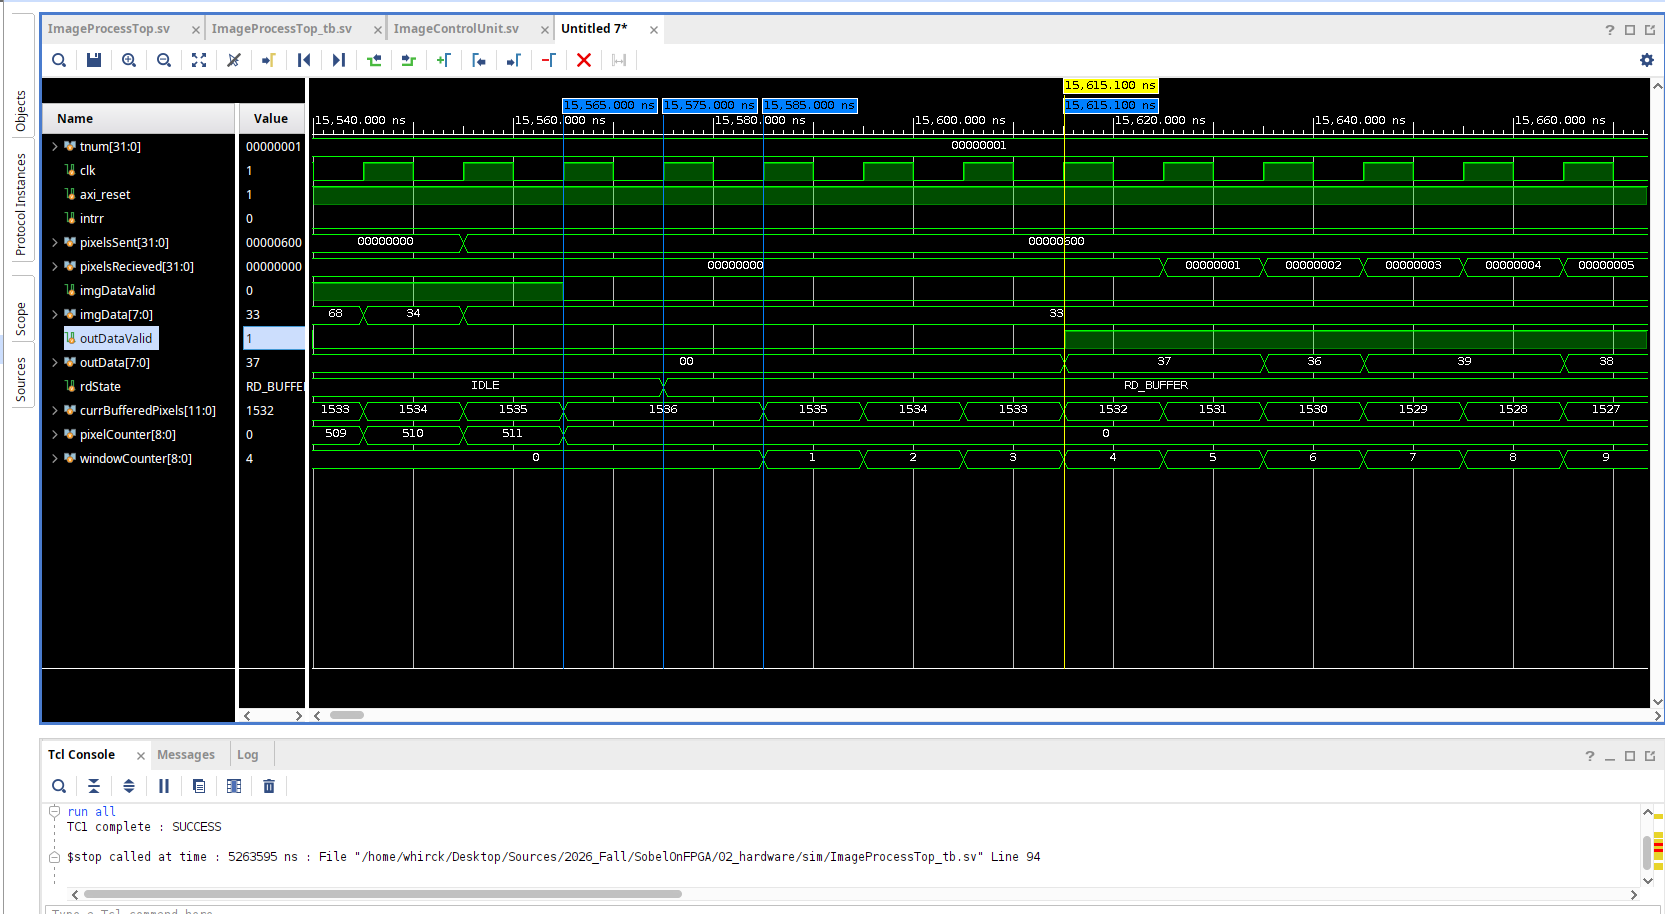
\includegraphics[
								width			= 0.8\textwidth,
								keepaspectratio	= true
							]{../01_supporting/image_control_unit_top/sim_3LB_start.png}
							\caption{3 line buffers}
						\end{subfigure}
						\hfill
						\begin{subfigure}{1.0\textwidth}
							\centering
							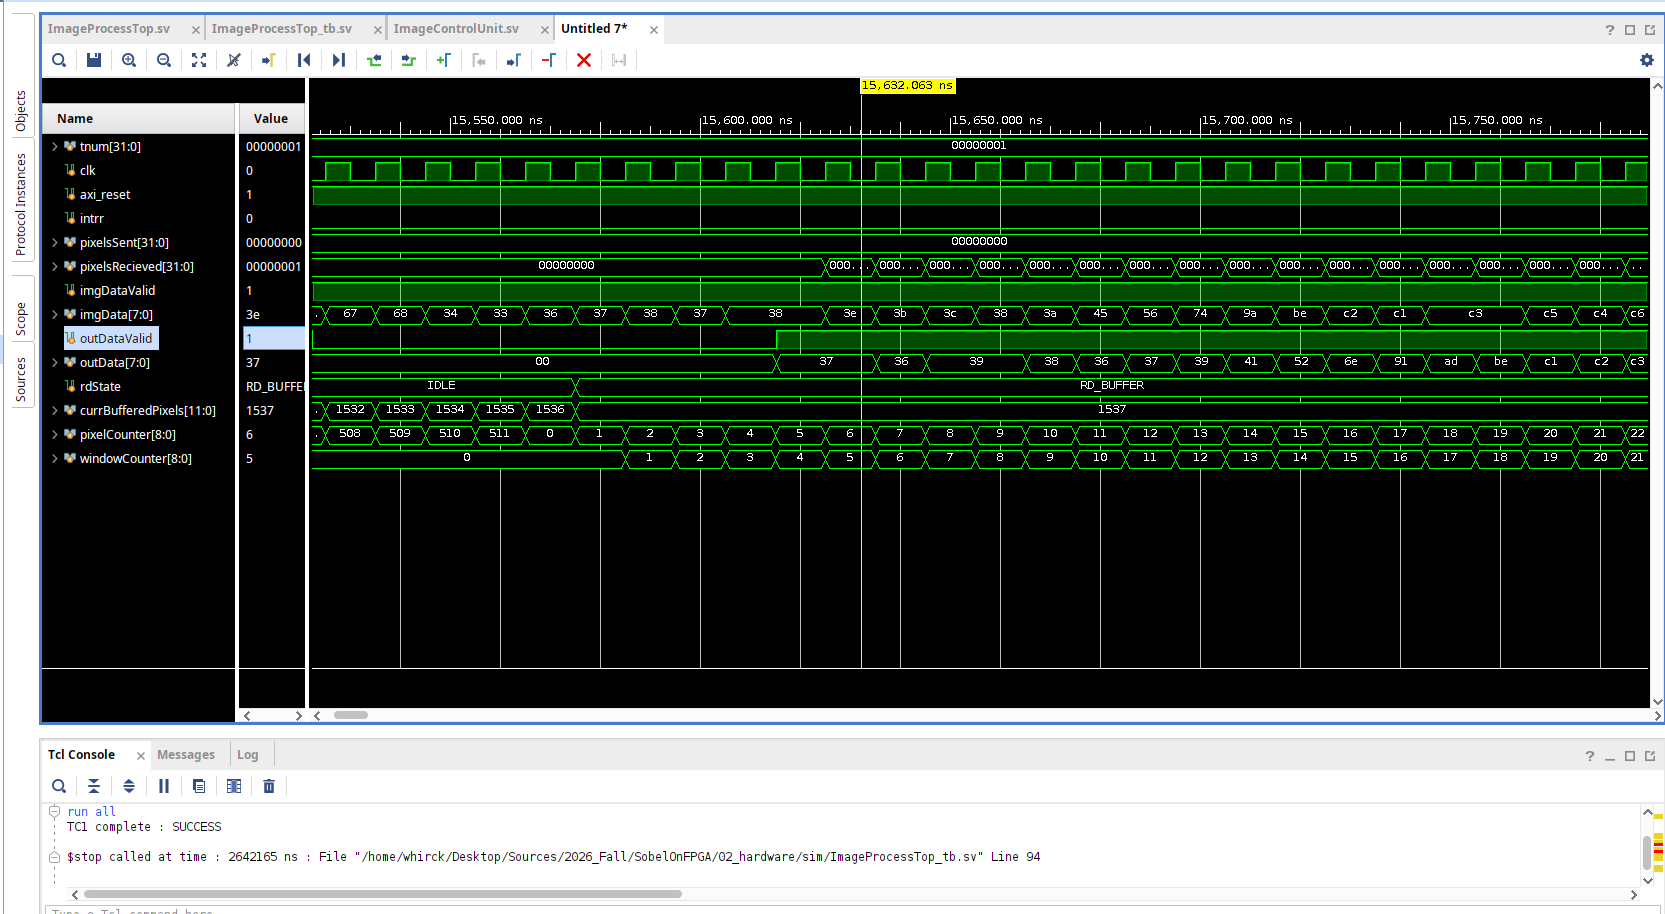
\includegraphics[
								width			= 0.8\textwidth,
								keepaspectratio	= true
							]{../01_supporting/image_control_unit_top/sim_4LB_start.png}
							\caption{4 line buffers}
						\end{subfigure}
						\caption{Simulation start between 3 and 4 prefilled LineBuffers}
						\label{fig:}
					\end{figure}	

					Observations between these starting waveforms:
					\begin{itemize}
						\item Both begin outputting result pixel data and reach 
								the \texttt{RD\_BUFFER} state. 
						\item Only 4LB accepts \texttt{imgData} by keeping \texttt{imgDataValid}
								high but 3LB lowers this signal. This is our 4th row
								being written to the buffer.
						\item Both waveforms reach a net buffer count of three rows (1536)
							in \texttt{currBufferedPixels} but the 3LB doesn't 
							retain this number. 3LB decreases in net pixel count because
							it is no longer importing data while exporting, something 
							of a triangle wave of net bufferd pixels. 
						\item No interrupt signals are present for both signals during this 
								startup. 
					\end{itemize}

					
					Lastly, lets consider the waveforms at the crossover between FSM logic.
					\begin{figure}[H]
						\centering
						\begin{subfigure}{1.0\textwidth}
							\centering
							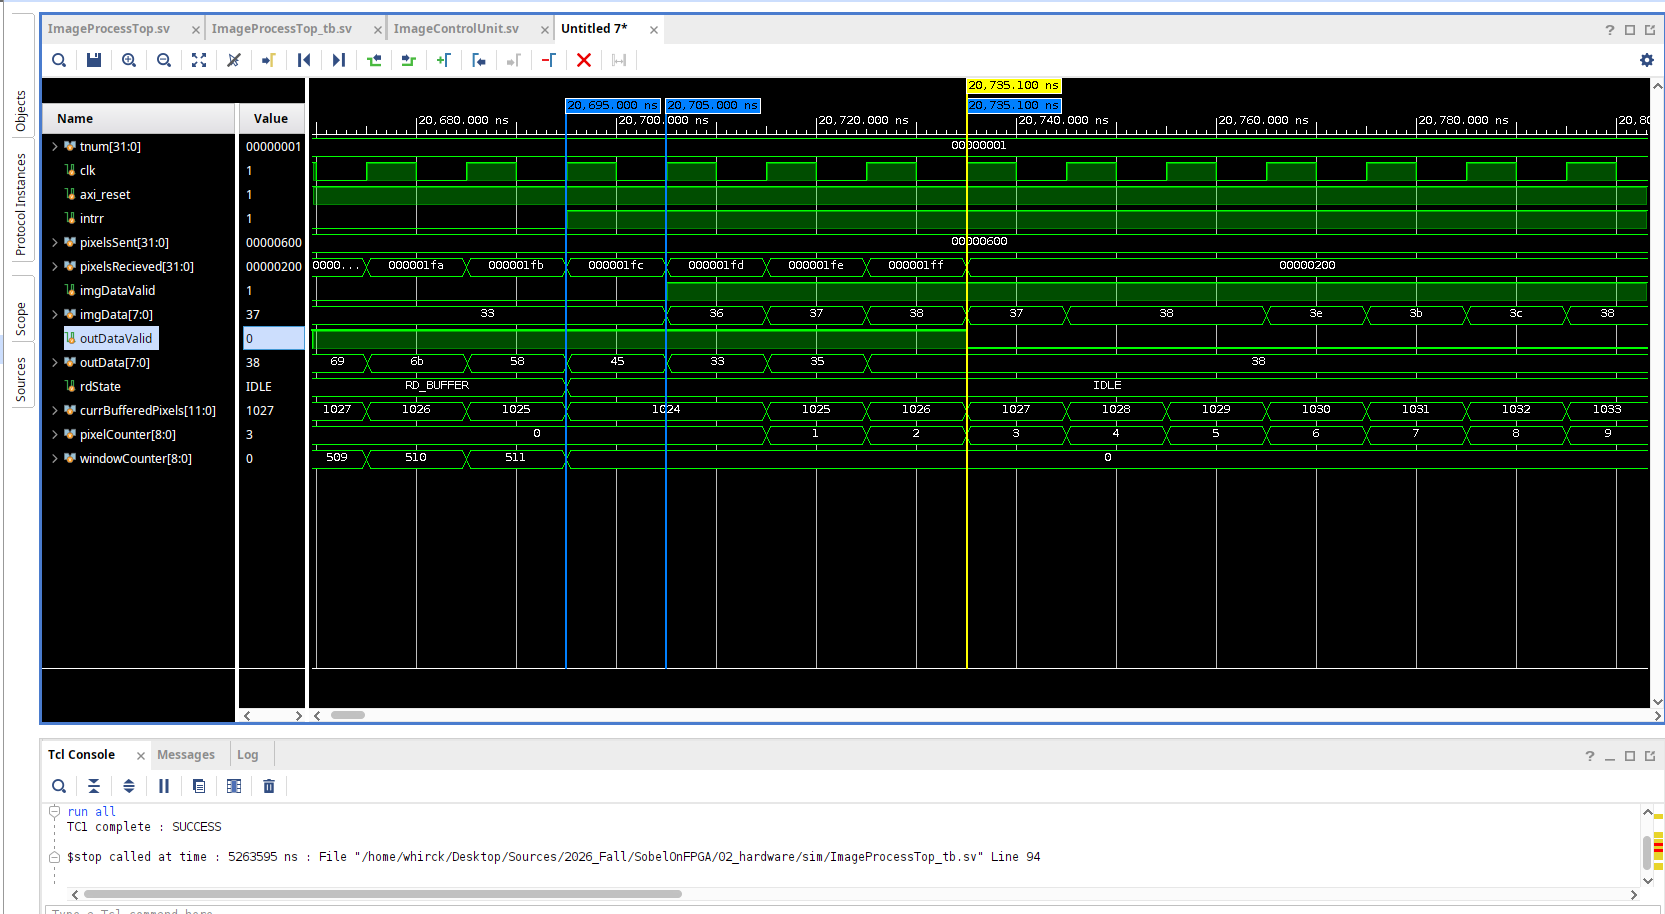
\includegraphics[
								width			= 0.8\textwidth,
								keepaspectratio	= true
							]{../01_supporting/image_control_unit_top/sim_3LB_crossover1.png}
							\caption{3 line buffers : RD to IDLE}
						\end{subfigure}
						\hfill
						\begin{subfigure}{1.0\textwidth}
							\centering
							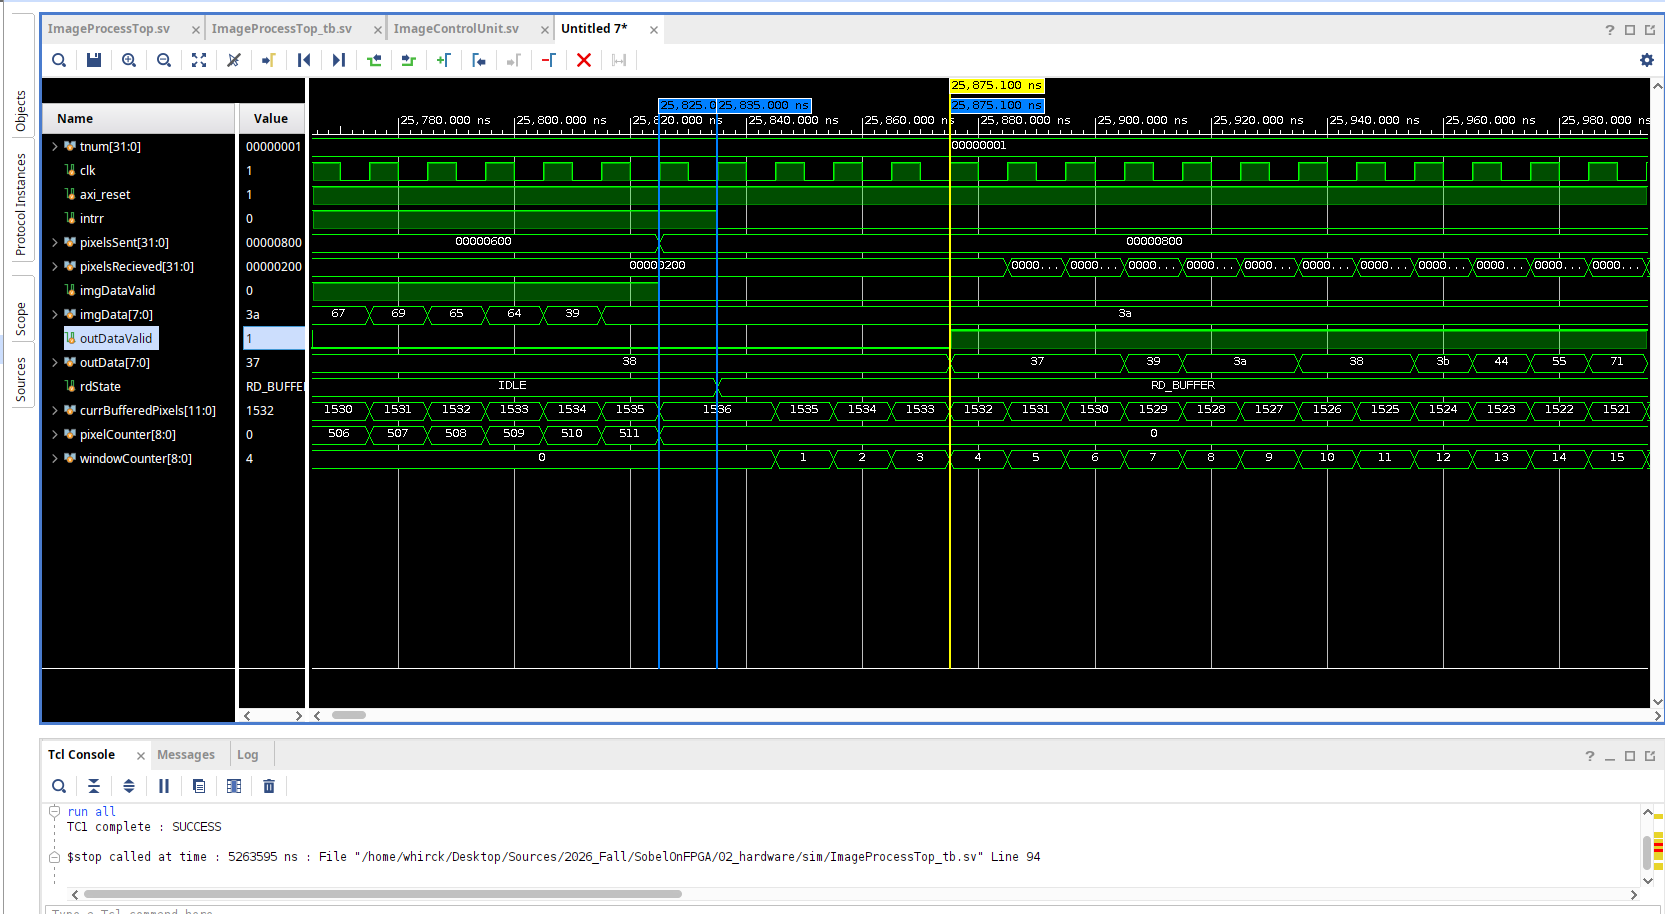
\includegraphics[
								width			= 0.8\textwidth,
								keepaspectratio	= true
							]{../01_supporting/image_control_unit_top/sim_3LB_crossover2.png}
							\caption{3 line buffers : IDLE to RD}
						\end{subfigure}
						\hfill
						\begin{subfigure}{1.0\textwidth}
							\centering
							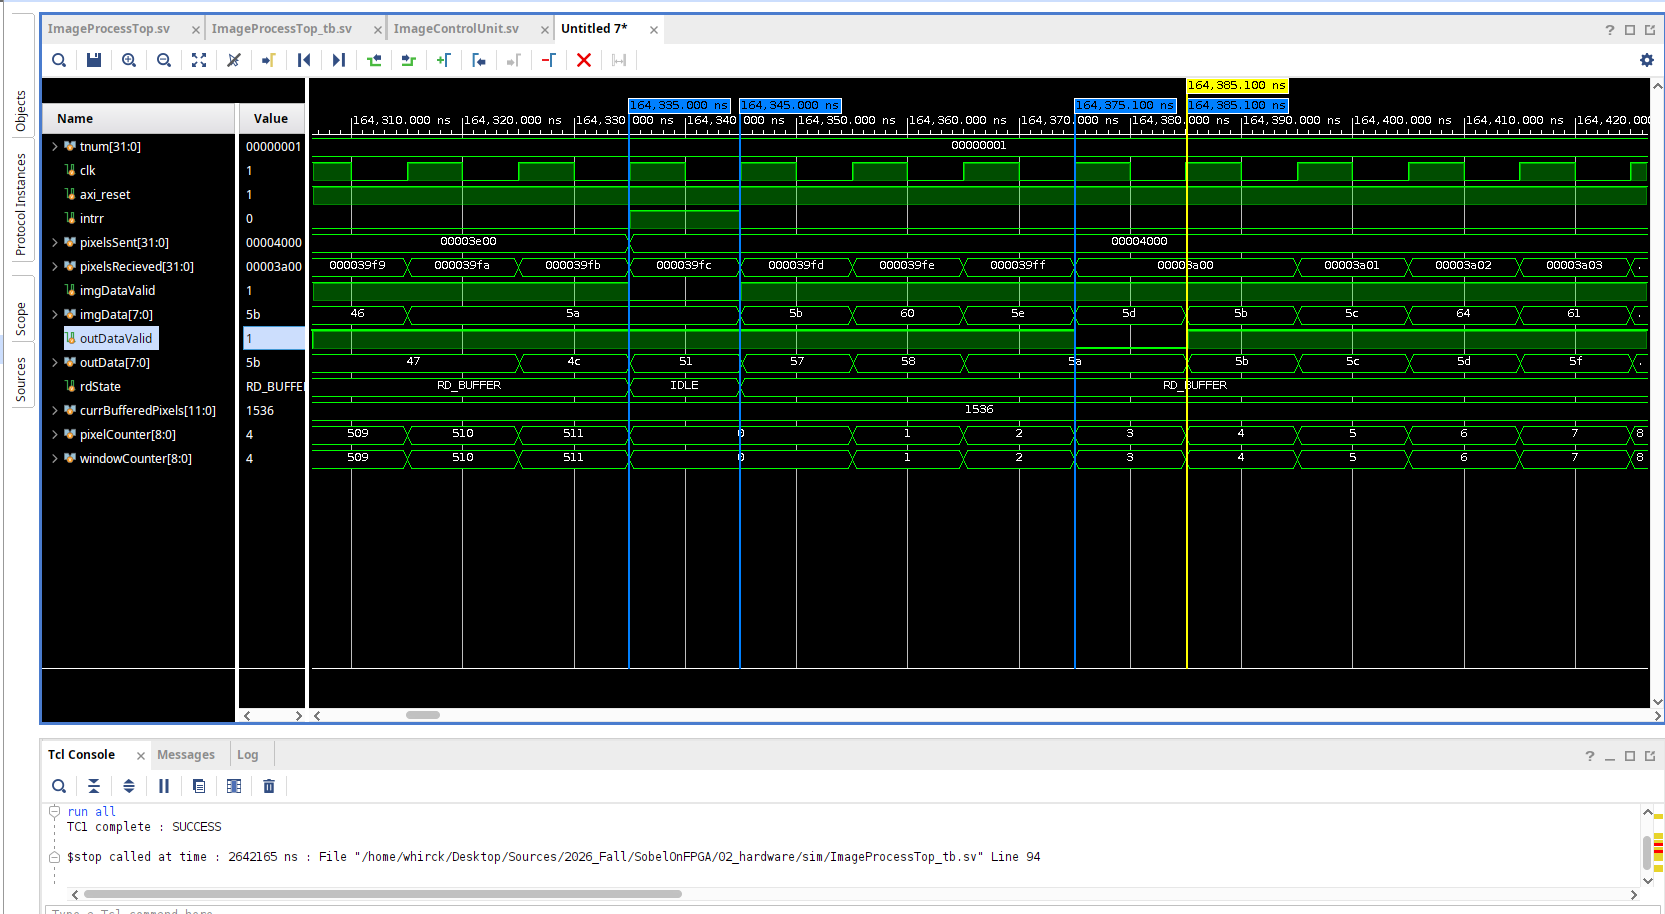
\includegraphics[
								width			= 0.8\textwidth,
								keepaspectratio	= true
							]{../01_supporting/image_control_unit_top/sim_4LB_crossover.png}
							\caption{4 line buffers}
						\end{subfigure}
						\caption{Simulation start between 3 and 4 prefilled LineBuffers}
						\label{fig:}
					\end{figure}	


			\subsection{Testing}

				The kernel used was the box blur which averages all neighboring
				pixels with a gain of 1.
				\[
					K = 
					\frac{1}{9}
					\begin{bmatrix}
						1 & 1 & 1 \\
						1 & 1 & 1 \\
						1 & 1 & 1 
					\end{bmatrix}
				\] 
	
				\begin{figure}[H]
					\centering
					\begin{subfigure}{0.4\textwidth}
						\centering
						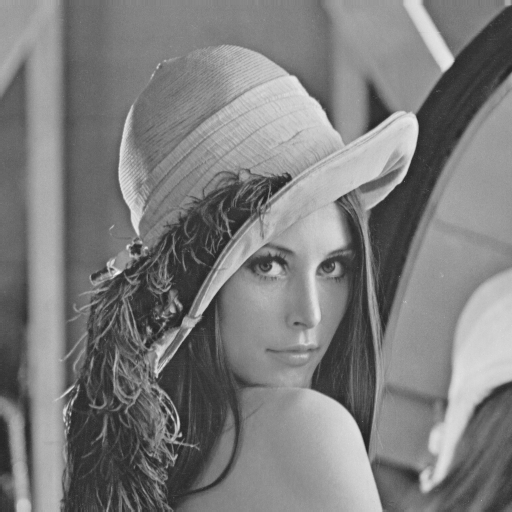
\includegraphics[
							width			= \textwidth,
							keepaspectratio	= true
						]{../01_supporting/image_control_unit_top/testimg1.png}
						\caption{Input Image}
					\end{subfigure}
					%\hfill
					\begin{subfigure}{0.4\textwidth}
						\centering
						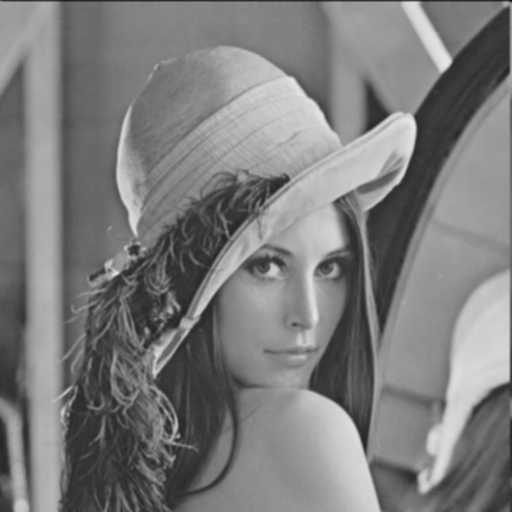
\includegraphics[
							width			= \textwidth,
							keepaspectratio	= true
						]{../01_supporting/image_control_unit_top/blurred_testimg1.png}
						\caption{Output Filtered Image}
					\end{subfigure}
					%\hfill
					\begin{subfigure}{0.4\textwidth}
						\centering
						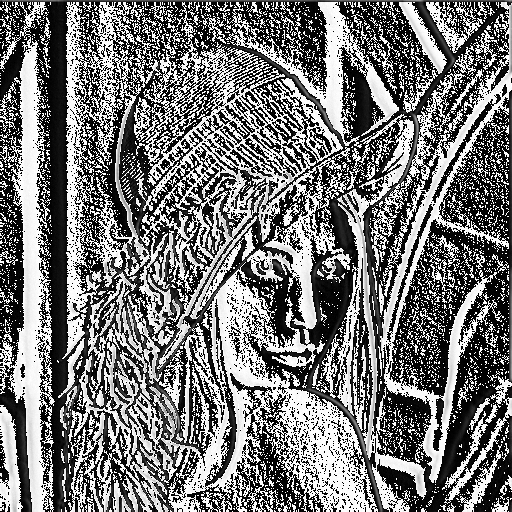
\includegraphics[
							width			= \textwidth,
							keepaspectratio	= true
						]{../01_supporting/image_control_unit_top/diff_testimg1.png}
						\caption{Difference Image (shift unfixed)}
					\end{subfigure}
					%\hfill
					\begin{subfigure}{0.4\textwidth}
						\centering
						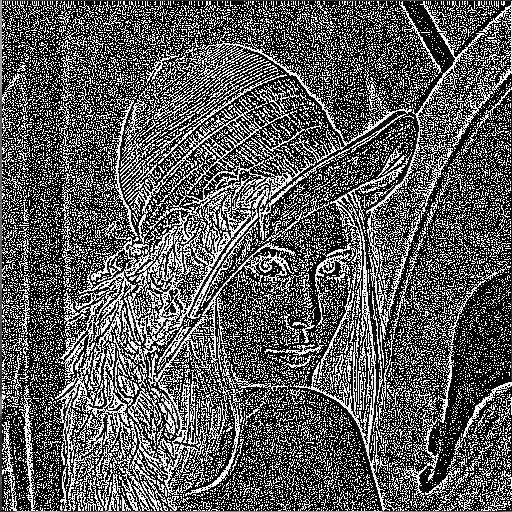
\includegraphics[
							width			= \textwidth,
							keepaspectratio	= true
						]{../01_supporting/image_control_unit_top/diff_testimg1_shiftfix.png}
						\caption{Difference Image (shift fixed)}
					\end{subfigure}
					\caption{I/O of image}
					\label{fig:result_imtop}
				\end{figure}	

				\begin{figure}[H]
					\centering
					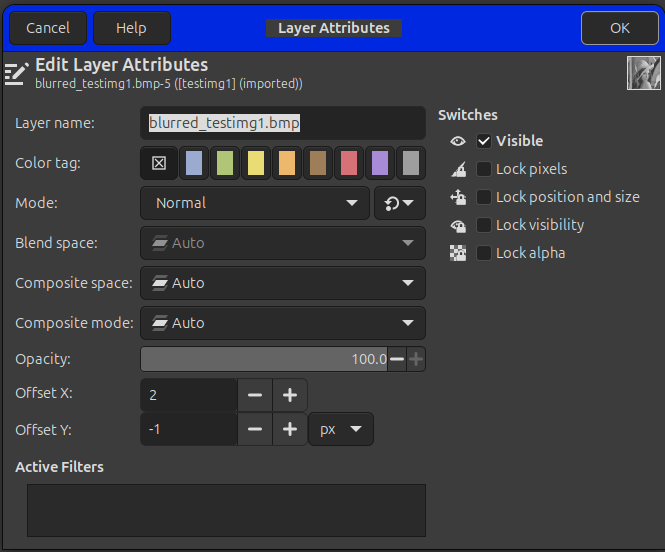
\includegraphics[
						width			= 0.5\textwidth,
						keepaspectratio	= true
					]{../01_supporting/image_control_unit_top/pixel_offset.png}
					\caption{Offset on Output Image}
				\end{figure}

				Observations
				\begin{itemize}
					\item Output image (b) is blurred
					\item Output image (b) has a black pixel boarder
						on the top and right sides of the picture.
					\item Difference image (d) gives a much better
						depiction of the high-frequency details that were
						removed than image (c). The pixels are also uniform
						throughout the image as well, which is not the case
						in (c). 
				\end{itemize}

			\subsection{Result Questions}

				\subsubsection{Q:Why was the entire output image shifted?}

			


	\chapter{Results}

	\chapter{Analysis}

	\chapter{Conclusion}

	\chapter{Appendix}
		\section{SystemVerilog}

			\subsection{Line Buffer}
	
				\lstinputlisting[
					language	= {Verilog},
					captionpos	= top,
					caption		= {\texttt{LineBuffer.sv}},
					breaklines	= true,
					label		= {code:linebuff}
				]{../02_hardware/src/LineBuffer.sv}

				\lstinputlisting[
					language	= {Verilog},
					captionpos	= top,
					caption		= {\texttt{LineBuffer\_tb.sv}},
					breaklines	= true,
					label		= {testcode:linebuff}
				]{../02_hardware/sim/LineBuffer_tb.sv}


			\subsection{Convolution}
	
				\lstinputlisting[
					language	= {Verilog},
					captionpos	= top,
					caption		= {\texttt{Convolution.sv}},
					breaklines	= true,
					label		= {code:convolution}
				]{../02_hardware/src/Convolution.sv}

				\lstinputlisting[
					language	= {Verilog},
					captionpos	= top,
					caption		= {\texttt{Convolution\_tb.sv}},
					breaklines	= true,
					label		= {testcode:convolution}
				]{../02_hardware/sim/Convolution_tb.sv}


			\subsection{Image Control Unit}
	
				\lstinputlisting[
					language	= {Verilog},
					captionpos	= top,
					caption		= {\texttt{ImageControlUnit.sv}},
					breaklines	= true,
					label		= {code:imu}
				]{../02_hardware/src/ImageControlUnit.sv}

				\lstinputlisting[
					language	= {Verilog},
					captionpos	= top,
					caption		= {\texttt{ImageControlUnit\_tb.sv}},
					breaklines	= true,
					label		= {testcode:imu}
				]{../02_hardware/sim/ImageControlUnit_tb.sv}


	\chapter{References}
		\href{https://www.youtube.com/watch?v=Zm3KzhahbUg&list=PL1tvZA53A9hJnwmiqPt1KeXrAQ9kd52H2&index=11}{Youtube Inspiration}

\end{document}
